\documentclass[12pt,a4paper]{extarticle}
\usepackage[utf8]{inputenc}
\usepackage[T5]{fontenc}
\usepackage{geometry}
\geometry{a4paper, left=1.5cm, right=1cm, top=1.5cm, bottom=1.5cm, headheight=20pt, headsep=15pt, footskip=28pt}
\usepackage{enumitem}
\usepackage{amssymb}
\usepackage{setspace}
\usepackage{tikz}
\definecolor{book}{RGB}{58,90,172}
\newcommand{\noteicon}{\textcolor{book}{$\blacktriangleright$}}
\usetikzlibrary{patterns, patterns.meta, calc} % Thêm patterns.meta vào đây
% Gọi package nằm trong thư mục con template
\usepackage{../template/mngocbox}

\begin{document}
\onehalfspacing

% Sử dụng ngoặc vuông [...] để thay đổi linh hoạt các thông số
\makeheadbox[headerright={Tổng ôn 10-11},chude={CHỦ ĐỀ 04},tieude={Oxy, ba đường conic},dinhdang={Hình học},lop={12 },gv={Nguyễn Lê Minh Ngọc}]

\vspace{2em}
\makeheading{I}{Tóm tắt lý thuyết}
\section{Phương trình đường thẳng}
\subsection{Phương trình tổng quát của đường thẳng}
\begin{minipage}{0.65\textwidth}
Vectơ $\vec{n}$ được gọi là vectơ pháp tuyến của đường thẳng $\Delta$ nếu $\vec{n} \ne \vec{0}$ có giá của vectơ $\vec{n}$ vuông góc với $\Delta$.
\smallskip
\textcolor{book}{$\blacktriangleright$} \textbf{Nhận xét:}
\begin{itemize}
    \item Nếu $\vec{n}$ là một vectơ pháp tuyến của $\Delta$ khi $k\vec{n}$ ($k \ne 0$) cũng là một vectơ pháp tuyến của $\Delta$.
    \item Một đường thẳng hoàn toàn được xác định khi biết một điểm và một vectơ pháp tuyến của đường thẳng đó.
\end{itemize}
\end{minipage}
\hfill
\begin{minipage}{0.3\textwidth}
\centering
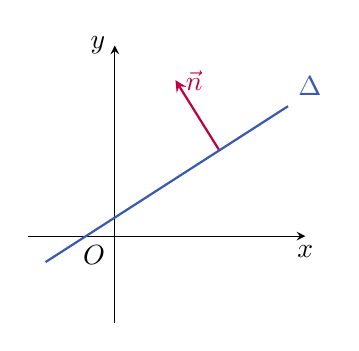
\begin{tikzpicture}[scale=1.1, >=stealth]
    % Trục tọa độ
    \draw[->] (-1,0) -- (2.2,0) node[below] {$x$};
    \draw[->] (0,-1) -- (0,2.2) node[left] {$y$};
    \node[below left] at (0,0) {$O$};
    % Đường thẳng Delta
    \draw[thick, book] (-0.8, -0.3) -- (2.0, 1.5) node[above right] {$\Delta$};
    % Vectơ n pháp tuyến
    \draw[->, thick, purple] (1.2, 1.0) -- (0.7, 1.8) node[right] {$\vec{n}$};
\end{tikzpicture}
\end{minipage}
\vspace{0.5cm}
\begin{minipage}{0.65\textwidth}
Trong mặt phẳng toạ độ, mọi đường thẳng đều có \textcolor{book}{phương trình tổng quát} dạng \textcolor{book}{$ax + by + c = 0$}, với $a$ và $b$ không đồng thời bằng $0$. Ngược lại, mỗi phương trình dạng $ax + by + c = 0$, với $a$ và $b$ không đồng thời bằng $0$, đều là phương trình của một đường thẳng, nhận \textcolor{book}{$\vec{n}(a; b)$} là một \textcolor{book}{vectơ pháp tuyến}.
\end{minipage}
\hfill
\begin{minipage}{0.3\textwidth}
\centering
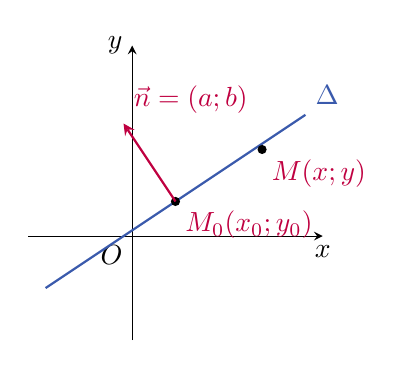
\begin{tikzpicture}[scale=1.1, >=stealth]
    % Trục tọa độ
    \draw[->] (-1.2,0) -- (2.2,0) node[below] {$x$};
    \draw[->] (0,-1.2) -- (0,2.2) node[left] {$y$};
    \node[below left] at (0,0) {$O$};
    % Đường thẳng Delta
    \draw[thick, book] (-1.0, -0.6) -- (2.0, 1.4) node[above right] {$\Delta$};
    % Điểm M0 và M
    \fill (0.5, 0.4) circle (1.5pt) node[below right, purple] {$M_0(x_0; y_0)$};
    \fill (1.5, 1.0) circle (1.5pt) node[below right, purple] {$M(x; y)$};
    % Vectơ n pháp tuyến xuất phát từ M0
    \draw[->, thick, purple] (0.5, 0.4) -- (-0.1, 1.3) node[above right] {$\vec{n} = (a; b)$};
\end{tikzpicture}
\end{minipage}
\vspace{0.5cm}
\textcolor{book}{$\blacktriangleright$} \textbf{Nhận xét:} Trong mặt phẳng toạ độ, cho đường thẳng $\Delta: ax + by + c = 0$.
\begin{itemize}
    \item Nếu $b = 0$ thì phương trình $\Delta$ có thể đưa về dạng $x = m$ $\left( m = -\dfrac{c}{a} \right)$ và $\Delta$ vuông góc với $Ox$.
    \item Nếu $b \ne 0$ thì phương trình $\Delta$ có thể đưa về dạng $y = nx + p$ $\left( n = -\dfrac{a}{b}; p = -\dfrac{c}{b} \right)$.
\end{itemize}
\vspace{0.5cm}
\subsection*{\textcolor{book}{1.2 Phương trình tham số của đường thẳng}}
\begin{minipage}{0.65\textwidth}
Vectơ $\vec{u}$ được gọi là vectơ chỉ phương của đường thẳng $\Delta$ nếu $\vec{u} \ne \vec{0}$ và giá của $\vec{u}$ song song hoặc trùng với $\Delta$.
\smallskip
\textcolor{book}{$\blacktriangleright$} \textbf{Nhận xét:}
\begin{itemize}
    \item Nếu $\vec{u}$ là một vectơ chỉ phương của $\Delta$ thì $k\vec{u}$ ($k \ne 0$) cũng là một vectơ chỉ phương của $\Delta$.
    \item Một đường thẳng hoàn toàn xác định khi biết một điểm và một vectơ chỉ phương của đường thẳng đó.
\end{itemize}
\end{minipage}
\hfill
\begin{minipage}{0.3\textwidth}
\centering
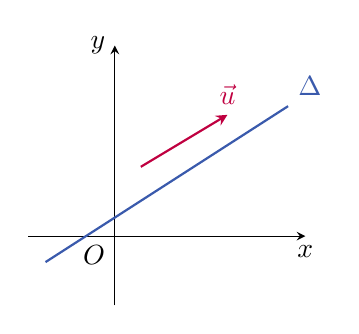
\begin{tikzpicture}[scale=1.1, >=stealth]
    % Trục tọa độ
    \draw[->] (-1,0) -- (2.2,0) node[below] {$x$};
    \draw[->] (0,-0.8) -- (0,2.2) node[left] {$y$};
    \node[below left] at (0,0) {$O$};
    % Đường thẳng Delta
    \draw[thick, book] (-0.8, -0.3) -- (2.0, 1.5) node[above right] {$\Delta$};
    % Vectơ u chỉ phương
    \draw[->, thick, purple] (0.3, 0.8) -- (1.3, 1.4) node[above] {$\vec{u}$};
\end{tikzpicture}
\end{minipage}
\begin{minipage}{0.65\textwidth}
Cho đường thẳng $\Delta$ đi qua điểm $A(x_0; y_0)$ và có vectơ chỉ phương $\vec{u}(a; b)$. Khi đó điểm $M(x; y)$ thuộc đường thẳng $\Delta$ khi và chỉ khi tồn tại số thực $t$ sao cho $\overrightarrow{AM} = t\vec{u}$, hay $\begin{cases} x = x_0 + at \\ y = y_0 + bt \end{cases}$
\medskip
Hệ trên được gọi là \textcolor{book}{phương trình tham số} của đường thẳng $\Delta$ ($t$ là tham số).
\end{minipage}
\hfill
\begin{minipage}{0.3\textwidth}
\centering
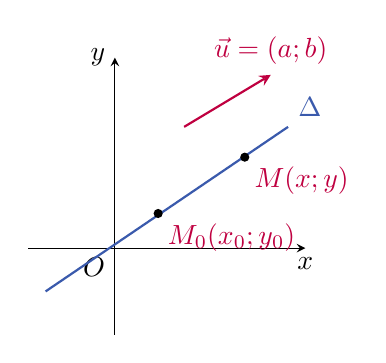
\begin{tikzpicture}[scale=1.1, >=stealth]
    % Trục tọa độ
    \draw[->] (-1,0) -- (2.2,0) node[below] {$x$};
    \draw[->] (0,-1) -- (0,2.2) node[left] {$y$};
    \node[below left] at (0,0) {$O$};
    % Đường thẳng Delta
    \draw[thick, book] (-0.8, -0.5) -- (2.0, 1.4) node[above right] {$\Delta$};
    % Các điểm
    \fill (0.5, 0.4) circle (1.5pt) node[below right, purple] {$M_0(x_0; y_0)$};
    \fill (1.5, 1.05) circle (1.5pt) node[below right, purple] {$M(x; y)$};
    % Vectơ u chỉ phương
    \draw[->, thick, purple] (0.8, 1.4) -- (1.8, 2.0) node[above] {$\vec{u} = (a; b)$};
\end{tikzpicture}
\end{minipage}
\vspace{0.4cm}
\textcolor{book}{$\blacklozenge$} 
\vspace{0.4cm}
\section*{\textcolor{book}{2. PHƯƠNG TRÌNH ĐƯỜNG TRÒN}}
\subsection*{\textcolor{book}{2.1 Phương trình đường tròn}}
\begin{minipage}{0.65\textwidth}
\textcolor{book}{\textbf{Phương trình đường tròn}}
Điểm $M(x; y)$ thuộc đường tròn $(C)$, tâm $I(a; b)$, bán kính $R$ khi và chỉ khi:
\[
(x - a)^2 + (y - b)^2 = R^2. \quad (1)
\]
Ta gọi (1) là phương trình của đường tròn $(C)$.
\end{minipage}
\hfill
\begin{minipage}{0.3\textwidth}
\centering
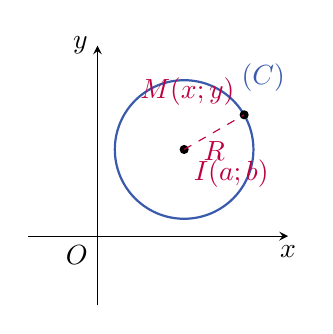
\begin{tikzpicture}[scale=1.1, >=stealth]
    % Trục tọa độ
    \draw[->] (-0.8,0) -- (2.2,0) node[below] {$x$};
    \draw[->] (0,-0.8) -- (0,2.2) node[left] {$y$};
    \node[below left] at (0,0) {$O$};
    % Đường tròn (C)
    \draw[thick, book] (1.0, 1.0) circle (0.8) node[above right=0.6cm] {$(C)$};
    % Tâm I và điểm M
    \fill (1.0, 1.0) circle (1.5pt) node[below right, purple] {$I(a; b)$};
    \coordinate (M) at ($(1.0, 1.0) + (30:0.8)$);
    \fill (M) circle (1.5pt) node[above left, purple] {$M(x; y)$};
    % Bán kính R
    \draw[dashed, purple] (1.0, 1.0) -- (M) node[midway, below] {$R$};
\end{tikzpicture}
\end{minipage}
\vspace{0.3cm}
\textcolor{book}{$\blacktriangleright$} \textbf{Nhận xét:} Phương trình (1) tương đương với $x^2 + y^2 - 2ax - 2by + (a^2 + b^2 - R^2) = 0$.
\vspace{0.3cm}
Phương trình $x^2 + y^2 - 2ax - 2by + c = 0$ là phương trình của một đường tròn $(C)$ khi và chỉ khi $a^2 + b^2 - c > 0$. Khi đó, $(C)$ có tâm $I(a; b)$ và bán kính $R = \sqrt{a^2 + b^2 - c}$.
\vspace{0.3cm}
\textcolor{book}{$\blacklozenge$} 
\vspace{0.4cm}
\subsection*{\textcolor{book}{2.2 Phương trình tiếp tuyến của đường tròn}}
Cho điểm $M(x_0; y_0)$ thuộc đường tròn $(C): (x - a)^2 + (y - b)^2 = R^2$ (tâm $I(a; b)$, bán kính $R$). Khi đó, tiếp tuyến $\Delta$ của $(C)$ tại $M(x_0; y_0)$ có vectơ pháp tuyến $\overrightarrow{MI} = (a - x_0; b - y_0)$ và phương trình:
\[
(a - x_0)(x - x_0) + (b - y_0)(y - y_0) = 0.
\]
\begin{center}
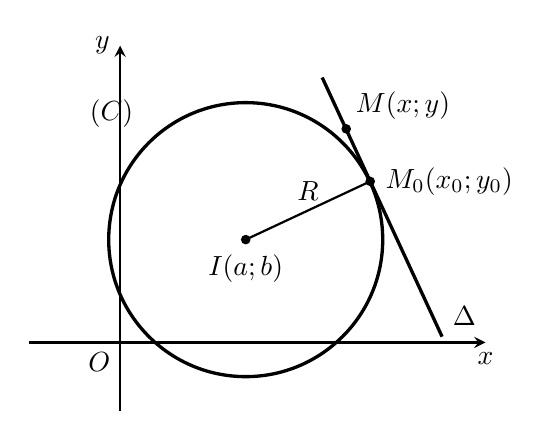
\begin{tikzpicture}[scale=1.45, >=stealth]
    % Trục tọa độ x, y dùng màu  có sẵn
    \draw[->, thick] (-0.8, 0) -- (3.2, 0) node[below] {$x$};
    \draw[->, thick] (0, -0.6) -- (0, 2.6) node[left] {$y$};
    \node[below left] at (0, 0) {$O$};
    
    % Đường tròn (C) tâm I(1.1; 0.9), bán kính R = 1.2
    \coordinate (I) at (1.1, 0.9);
    \draw[very thick] (1.1, 0.9) circle (1.2);
    \fill (I) circle (1.2pt) node[below=2pt] {$I(a; b)$};
    \node[above left] at (0.2, 1.8) {$(C)$};
    
    % Tiếp điểm M0(x0; y0) cố định bằng tọa độ tuyệt đối
    \coordinate (M0) at (2.19, 1.41);
    \fill (M0) circle (1.2pt) node[right=2pt] {$M_0(x_0; y_0)$};
    
    % Đoạn thẳng bán kính R nối từ I đến M0
    \draw[thick] (I) -- (M0) node[midway, above] {$R$};
    
    % ĐƯỜNG TIẾP TUYẾN Delta (Được vẽ bằng tọa độ tuyệt đối không lỗi)
    \draw[very thick] (1.77, 2.32) -- (2.82, 0.05) node[above right] {$\Delta$};
    
    % Điểm M(x; y) trên tiếp tuyến
    \coordinate (M) at (1.98, 1.87);
    \fill (M) circle (1.2pt) node[above right] {$M(x; y)$};
\end{tikzpicture}
\end{center}
\vspace{0.4cm}
\textcolor{book}{$\blacklozenge$} 
\subsection*{2.3 Góc giữa hai đường thẳng}
Hai đường thẳng cắt nhau tạo thành bốn góc, số đo của góc không tù được gọi là số đo góc (hay đơn giản là góc) giữa hai đường thẳng.
Góc giữa hai đường thẳng song song hoặc trùng nhau được quy ước bằng $0^\circ$.
\vspace{0.4cm}
Cho hai đường thẳng:
\[
\Delta_1: a_1x + b_1y + c_1 = 0 \quad \text{và} \quad \Delta_2: a_2x + b_2y + c_2 = 0
\]
với các vectơ pháp tuyến $\vec{n}_1(a_1; b_1)$ và $\vec{n}_2(a_2; b_2)$ tương ứng. Khi đó, góc $\varphi$ giữa hai đường thẳng đó được xác định thông qua công thức:
\[
\cos\varphi = \left| \cos(\vec{n}_1, \vec{n}_2) \right| = \frac{|\vec{n}_1 \cdot \vec{n}_2|}{|\vec{n}_1| \cdot |\vec{n}_2|} = \frac{|a_1a_2 + b_1b_2|}{\sqrt{a_1^2 + b_1^2} \cdot \sqrt{a_2^2 + b_2^2}}
\]
\vspace{0.3cm}
\noteicon \textbf{Chú ý:}
\begin{itemize}
    \item $\Delta_1 \perp \Delta_2 \Leftrightarrow \vec{n}_1 \perp \vec{n}_2 \Leftrightarrow a_1a_2 + b_1b_2 = 0$.
    \item Nếu $\Delta_1, \Delta_2$ có các vectơ chỉ phương $\vec{u}_1, \vec{u}_2$ thì góc $\varphi$ giữa $\Delta_1$ và $\Delta_2$ cũng được xác định thông qua công thức $\cos\varphi = \left| \cos(\vec{u}_1, \vec{u}_2) \right|$.
\end{itemize}
\vspace{0.3cm}
\vspace{0.5cm}
\subsection*{2.4 Khoảng cách từ một điểm đến một đường thẳng}
Trong trường hợp tổng quát, ta có:
\vspace{0.3cm}
Trong mặt phẳng tọa độ $Oxy$, cho đường thẳng $\Delta$ có phương trình $ax + by + c = 0$ ($a^2 + b^2 > 0$) và điểm $M(x_0; y_0)$. Khoảng cách từ điểm $M$ đến đường thẳng $\Delta$ ký hiệu là $d(M,\Delta)$, được tính bởi công thức như sau:\[
    d(M,\Delta) = \frac{|ax_0+by_0+c|}{\sqrt{a^2 + b^2}}
    \]
\textbf{Chú ý: } Nếu $M \in \Delta$ thì $d(M,\Delta)=0$ 
\section*{\textcolor{book}{3. Ba đường Conic}}
\subsection*{A. ĐƯỜNG ELIP}
\textbf{Định nghĩa}
Cho hai điểm $F_1, F_2$ cố định có khoảng cách $F_1F_2 = 2c$ ($c > 0$).\\
\vspace{0.5cm}
\textit{Đường elip} (còn gọi là elip) là tập hợp các điểm $M$ trong mặt phẳng sao cho $MF_1 + MF_2 = 2a$, trong đó $a$ là số cho trước lớn hơn $c$. Hai điểm $F_1$ và $F_2$ được gọi là hai \textbf{tiêu điểm} của elip.
% --- ĐỒ THỊ ELIP ---
\begin{center}
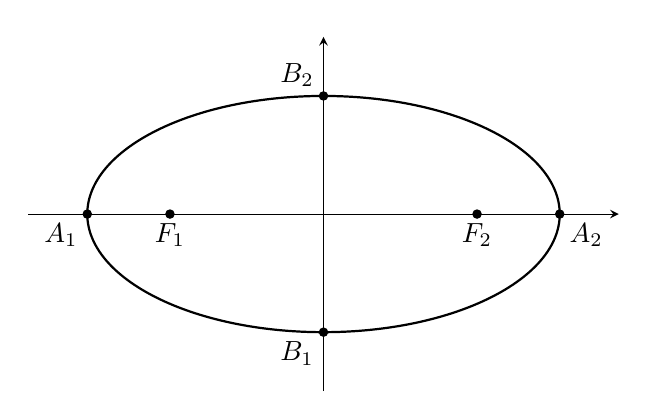
\begin{tikzpicture}[>=stealth, scale=1.5]
    % Hệ trục tọa độ (màu hồng/)
    \draw[->] (-2.5,0) -- (2.5,0) node[below] {};
    \draw[->] (0,-1.5) -- (0,1.5) node[left] {};
    
    % Đường Elip
    \draw[thick] (0,0) ellipse (2cm and 1cm);
    
    % Tiêu điểm và các đỉnh
    \filldraw (-1.3,0) circle (1pt) node[below] {$F_1$};
    \filldraw (1.3,0) circle (1pt) node[below] {$F_2$};
    \filldraw (-2,0) circle (1pt) node[below left] {$A_1$};
    \filldraw (2,0) circle (1pt) node[below right] {$A_2$};
    \filldraw (0,-1) circle (1pt) node[below left] {$B_1$};
    \filldraw (0,1) circle (1pt) node[above left] {$B_2$};
\end{tikzpicture}
\end{center}
\textbf{Phương trình chính tắc}
Trong mặt phẳng toạ độ $Oxy$, elip có hai tiêu điểm thuộc trục hoành sao cho $O$ là trung điểm của đoạn nối hai tiêu điểm đó, thì có phương trình
\[ \frac{x^2}{a^2} + \frac{y^2}{b^2} = 1, \text{ với } a > b > 0. \quad (1) \]
Ngược lại, mỗi phương trình có dạng (1), với $a > b > 0$, đều là phương trình của elip có hai tiêu điểm $F_1(-\sqrt{a^2 - b^2}; 0)$, $F_2(\sqrt{a^2 - b^2}; 0)$, tiêu cự $2c = 2\sqrt{a^2 - b^2}$ và tổng các khoảng cách từ mỗi điểm thuộc elip đó tới hai tiêu điểm bằng $2a$.
Phương trình (1) được gọi là \textbf{phương trình chính tắc} của elip tương ứng.
\vspace{0.5cm}
\subsection*{B. ĐƯỜNG HYPEBOL}
\noindent\textcolor{book}{\textbf{Định nghĩa đường hypebol}}
Cho hai điểm $F_1, F_2$ cố định có khoảng cách $F_1F_2 = 2c$ ($c > 0$).\\
\textit{Đường hypebol} (còn gọi là hypebol) là tập hợp các điểm $M$ sao cho $|MF_1 - MF_2| = 2a$, trong đó $a$ là số dương cho trước nhỏ hơn $c$. Hai điểm $F_1$ và $F_2$ được gọi là hai \textbf{tiêu điểm} của hypebol.
% --- ĐỒ THỊ HYPEBOL ---
\begin{center}
\begin{tikzpicture}[>=stealth, scale=1.5]
    % Hệ trục tọa độ (màu hồng/)
    \draw[->] (-2.5,0) -- (2.5,0) node[below] {$x$};
    \draw[->] (0,-1.5) -- (0,1.5) node[left] {$y$};
    \node[below left] at (0,0) {$O$};
    
    % Nhánh trái Hypebol
    \draw[thick, domain=-1.2:1.2, smooth, variable=\t] plot ({-0.8*sqrt(1 + \t*\t)}, \t);
    % Nhánh phải Hypebol
    \draw[thick, domain=-1.2:1.2, smooth, variable=\t] plot ({0.8*sqrt(1 + \t*\t)}, \t);
    
    % Tiêu điểm
    \filldraw (-1.5,0) circle (1pt) node[below] {$F_1$};
    \filldraw (1.5,0) circle (1pt) node[below] {$F_2$};
    
    % Điểm M và các đoạn thẳng MF1, MF2
    \coordinate (M) at (1.2, 0.75);
    \filldraw (M) circle (1pt) node[right] {$M(x; y)$};
    \draw (M) -- (-1.5,0);
    \draw (M) -- (1.5,0);
\end{tikzpicture}
\end{center}
\textbf{Phương trình chính tắc của đường hypebol}

Trong mặt phẳng toạ độ $Oxy$, hypebol có hai tiêu điểm thuộc trục hoành sao cho $O$ là trung điểm của đoạn nối hai tiêu điểm đó, thì có phương trình
\[ \frac{x^2}{a^2} - \frac{y^2}{b^2} = 1, \text{ với } a, b > 0. \quad (2) \]
Ngược lại, mỗi phương trình có dạng (2), với $a, b > 0$, đều là phương trình của hypebol có hai tiêu điểm $F_1(-\sqrt{a^2 + b^2}; 0)$, $F_2(\sqrt{a^2 + b^2}; 0)$, tiêu cự $2c = 2\sqrt{a^2 + b^2}$ và giá trị tuyệt đối của hiệu các khoảng cách từ mỗi điểm thuộc hypebol đến hai tiêu điểm bằng $2a$.
Phương trình (2) được gọi là \textbf{phương trình chính tắc} của hypebol tương ứng.
\vspace{0.5cm}
\subsection*{C. ĐƯỜNG PARABOL}
\textbf{Định nghĩa đường parabol}

Cho một điểm $F$ cố định và một đường thẳng $\Delta$ cố định không đi qua $F$.
\begin{itemize}
    \item Đường parabol (còn gọi là parabol) là tập hợp các điểm $M$ trong mặt phẳng cách đều $F$ và $\Delta$.
    \item Điểm $F$ được gọi là \textbf{tiêu điểm} của parabol. Đường thẳng $\Delta$ được gọi là \textbf{đường chuẩn} của parabol.
\end{itemize}

% --- ĐỒ THỊ PARABOL ---
\begin{center}
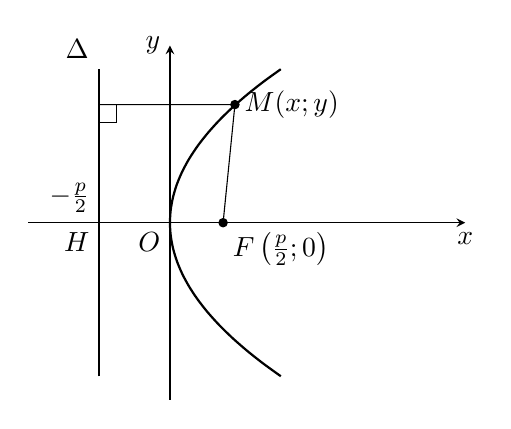
\begin{tikzpicture}[>=stealth, scale=1.5]
    % Hệ trục tọa độ (màu hồng/)
    \draw[->, ] (-1.2,0) -- (2.5,0) node[below] {$x$};
    \draw[->, ] (0,-1.5) -- (0,1.5) node[left] {$y$};
    \node[, below left] at (0,0) {$O$};
    
    % Đường chuẩn \Delta
    \draw[thick, ] (-0.6,-1.3) -- (-0.6,1.3) node[above left] {$\Delta$};
    \node[, below left] at (-0.6,0) {$H$};
    \node[, above left] at (-0.6,0) {$-\frac{p}{2}$};
    
    % Đường Parabol y^2 = 2px. Chọn p = 1.2 -> x = y^2 / 1.8
    \draw[thick, , domain=-1.3:1.3, smooth, variable=\y] plot ({\y*\y/1.8}, \y);
    
    % Tiêu điểm F
    \filldraw[] (0.45,0) circle (1pt) node[below right] {$F\left(\frac{p}{2}; 0\right)$};
    
    % Điểm M trên Parabol (chọn y = 1.0 -> x = 1/1.8 = 0.55)
    \coordinate (M) at (0.55, 1.0);
    \filldraw[] (M) circle (1pt) node[right] {$M(x;y)$};
    
    % Đoạn MF và đường vuông góc từ M đến \Delta
    \draw[] (M) -- (0.45,0);
    \draw[] (M) -- (-0.6,1.0);
    
    % Ký hiệu góc vuông tại giao điểm với đường chuẩn
    \draw[] (-0.6, 0.85) -- (-0.45, 0.85) -- (-0.45, 1.0);
\end{tikzpicture}
\end{center}
\textbf{Phương trình chính tắc của parabol}
Xét $(P)$ là một parabol với tiêu điểm $F$, đường chuẩn $\Delta$. Gọi $H$ là hình chiếu vuông góc của $F$ trên $\Delta$. Khi đó, trong hệ trục toạ độ $Oxy$ với gốc $O$ là trung điểm của $HF$, tia $Ox$ trùng tia $OF$, parabol $(P)$ có phương trình
\[ y^2 = 2px \text{ (với } p > 0). \quad (3) \]
Phương trình (3) được gọi là \textbf{phương trình chính tắc} của parabol $(P)$.
Ngược lại, mỗi phương trình dạng (3), với $p > 0$, là phương trình chính tắc của parabol có tiêu điểm $F\left(\frac{p}{2}; 0\right)$ và đường chuẩn $\Delta: x = -\frac{p}{2}$.\\
\vspace{0.5cm}
\makeheading{II}{Bài tập tự luyện}
\textbf{Câu 1.} Vectơ pháp tuyến của đường thẳng $2x - 3y + 6 = 0$ là:
A. $\vec{n} = (2;-3)$. \hfill
B. $\vec{n} = (2;3)$. \hfill
C. $\vec{n} = (3;2)$. \hfill
D. $\vec{n} = (-3;2)$.\\
\vspace{0.5cm}
\textbf{Câu 3.} Trong hệ trục $Oxy$ cho hai điểm $A(2; 1), B(2; 3)$ và $d: x + y - 4 = 0$. Tìm điểm $M$ thuộc $d$ sao cho $MA + MB$ nhỏ nhất?
A. $M(2; 2)$. \hfill
B. $M(1; 3)$. \hfill
C. $M(4; 0)$. \hfill
D. $M(-2; 6)$.\\
\vspace{0.5cm}
\textbf{Câu 5.} Việc quy đổi nhiệt độ giữa đơn vị độ C (Anders Celsius, 1701 - 1744) và đơn vị độ F (Daniel Fahrenheit, 1686 - 1736) được xác định bởi hai mốc sau: Nước đóng băng ở $0^\circ C, 32^\circ F$, nước sôi ở $100^\circ C, 212^\circ F$. Trong quy đổi đó, nếu $a^\circ C$ tương ứng với $b^\circ F$ thì trên mặt phẳng tọa độ $Oxy$, điểm $M(a,b)$ thuộc đường thẳng đi qua $A(0; 32)$ và $B(100; 212)$. Hỏi $0^\circ F$ và $100^\circ F$ tương ứng với bao nhiêu $^\circ C$:\\
\vspace{0.5cm}
\textbf{Câu 7.} Cho đường thẳng $d: \begin{cases} x = 2 + 2t \\ y = t \end{cases} (t \in \mathbb{R})$ và ba điểm $A(3; 4), B(-1; 2), C(0; 1)$. Điểm $M$ nằm trên đường thẳng $d$ sao cho $P = \left| \overrightarrow{MA} - 2\overrightarrow{MB} + 3\overrightarrow{MC} \right|$ nhỏ nhất có tọa độ là $(a; b)$.
Tính $T = a + 2b$.
$\Rightarrow$ Đáp số: ..........\\
\vspace{0.5cm}
\textbf{Câu 9.} Xét trên khu vực biển khá nhỏ ta xem mặt biển là một mặt phẳng. Đặt vào mặt phẳng ấy một hệ trục tọa độ $Oxy$, mỗi đơn vị trên trục ứng với 1 km. Có ba hòn đảo $A, B, C$ có tọa độ thỏa mãn $A(1; 2), \overrightarrow{AB} = (60; 80), \overrightarrow{AC} = (10; 10)$. Một chiếc tàu chở du khách từ đảo $A$ đến đảo $B$ để tham quan du lịch. Khi di chuyển thì du khách thấy đảo $C$ hiện ra thấp thoáng. Khoảng cách ngắn nhất từ chiếc tàu chở du khách đến đảo $C$ là bao nhiêu km?
$\Rightarrow$ Đáp số: ..........\\
\begin{center}
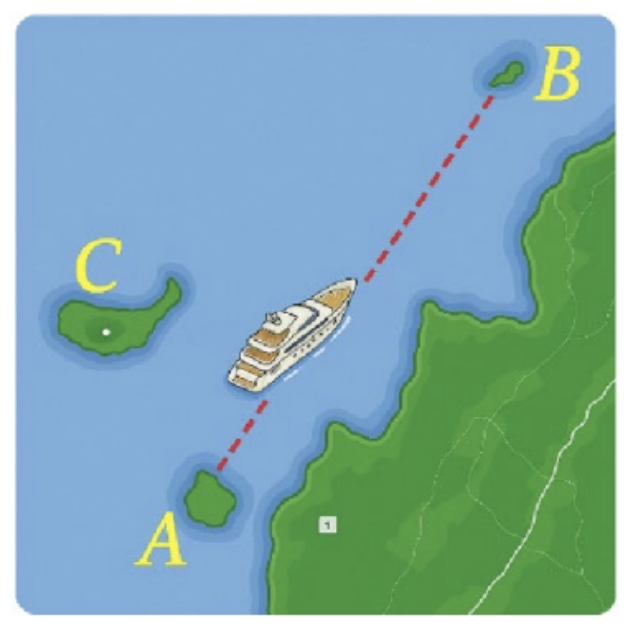
\includegraphics[width=0.3\textwidth]{5.9.png}
\end{center}
\textbf{Câu 1.} Câu lạc bộ bóng đá AS ROMA dự định xây dựng SVĐ mới có tên là Stadio Della Roma để làm sân nhà của đội bóng thay thế cho sân bóng Olimpico. Hệ thống mái của SVĐ Stadio Della Roma dự định được xây dựng có dạng hai hình elip như (hình 1) và được biểu diễn trên hệ trục tọa độ như (hình 2) với hình elip lớn bên ngoài có độ dài đoạn $A_1A_2 = 146$ mét, đoạn $B_1B_2 = 108$ mét, hình elip nhỏ bên trong có độ dài đoạn $A_3A_4 = 110$ mét và $B_3B_4 = 72$ mét. Xét tính đúng sai của các khẳng định sau:\\
a) Đường elip lớn trong hình 2 có phương trình chính tắc: $\dfrac{x^2}{5329} + \dfrac{y^2}{2916} = 1$.\\
b) Phương trình $1296x^2 + 3025y^2 = 3920400$ là phương trình của đường elip nhỏ trong hình 1.\\
c) Đường elip lớn trong hình 2 đã cho có một tiêu điểm $F_1(-\sqrt{2413}; 0)$.\\
d) Đường elip trong nhỏ hình 2 có tiêu cự $1729$.\\
\begin{center}
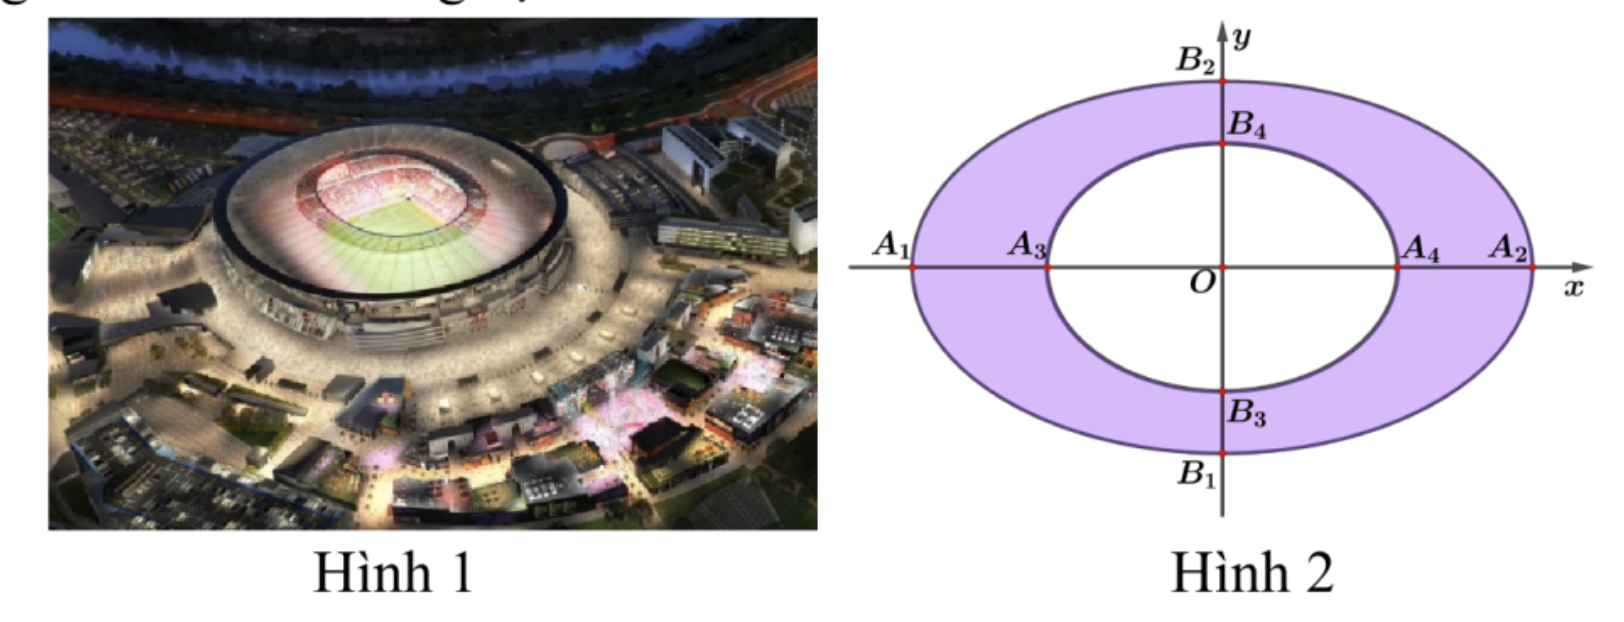
\includegraphics[width=0.5\textwidth]{6.1.png}
\end{center}
\vspace{0.5cm}
\vspace{0.5cm}
\textbf{Câu 3.} Điều hướng LORAN (điều hướng vô tuyến đường dài) cho máy bay và tàu thủy sử dụng các xung đồng bộ được truyền bởi hai trạm phát đặt cách xa nhau. Các xung này di chuyển với tốc độ ánh sáng ($186000$ dặm / giây). Sự chênh lệch về thời gian nhận được phản xạ của các xung này từ một máy bay hoặc tàu thủy là không đổi, nên máy bay hoặc con tàu sẽ nằm trên một hyperbol có các trạm phát là các tiêu điểm. Giả sử rằng hai trạm phát, cách nhau $300$ dặm, được đặt trên một hệ tọa độ vuông góc tại các điểm có tọa độ $(-150; 0)$ và $(150; 0)$ và một con tàu đang đi trên một con đường là một nhánh của hypebol và có tọa độ $(x; 75)$ (xem hình vẽ).\\
\begin{center}
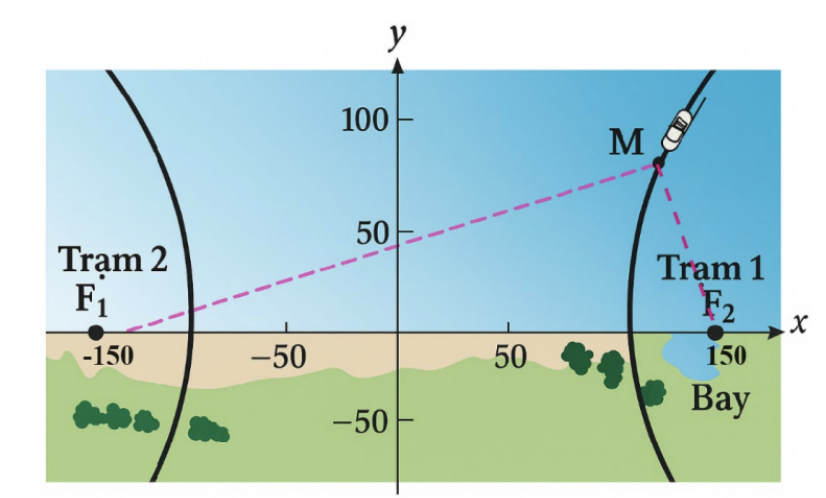
\includegraphics[width=0.5\textwidth]{6.3.png}
\end{center}
a) Tiêu cự của đường hypebol con tàu đi là $300$.\\
b) Hiệu khoảng cách tín hiệu giữa còn tàu và hai trạm phát là $93$ dặm.\\
c) Hypebol có phương trình $(H): \dfrac{x^2}{8649} + \dfrac{y^2}{13851} = 1$.\\
d) Hoành độ con tàu có giá trị gần bằng $110,3$.\\
\vspace{0.5cm}
\makeheading{III}{Bài tập làm thêm}
\textbf{Câu 2.} Vectơ nào dưới đây là một vectơ pháp tuyến của đường thẳng đi qua hai điểm $A(2; 3)$, và $B(4; 1)$?
A. $\vec{n} = (2;-2)$. \hfill
B. $\vec{n} = (2;-1)$. \hfill
C. $\vec{n} = (1;1)$. \hfill
D. $\vec{n} = (1;-2)$.
\\
\vspace{0.5cm}
\textbf{Câu 4.} Cho tam giác $ABC$ biết trực tâm $H(1; 1)$ và phương trình cạnh $AB: 5x - 2y + 6 = 0$, phương trình cạnh $AC: 4x + 7y - 21 = 0$. Phương trình cạnh $BC$ là
A. $4x - 2y + 1 = 0$. \hfill
B. $x - 2y + 14 = 0$. \hfill
C. $x + 2y - 14 = 0$. \hfill
D. $x - 2y - 14 = 0$.\\
\vspace{0.5cm}
\textbf{Câu 6.} Theo Google Maps, sân bay Nội Bài có vĩ độ là $21,2^\circ$ Bắc, kinh độ $105,8^\circ$ Đông, sân bay Đà Nẵng có vĩ độ là $16.1^\circ$ Bắc, kinh độ $108,2^\circ$ Đông. Một máy bay, bay từ Nội Bài đến sân bay Đà Nẵng. Tại thời điểm $t$ giờ, tính từ lúc xuất phát, máy bay ở vị trí có vĩ độ $x^\circ$ Bắc, kinh độ $y^\circ$ Đông được tính theo công thức $\begin{cases} x = 21,2 - \dfrac{153}{40}t \\ y = 105,8 + \dfrac{9}{5}t \end{cases}$. Hỏi chuyến bay từ Hà Nội đến Đà Nẵng mất bao nhiêu phút?
$\Rightarrow$ Đáp số: ..........\\
\vspace{0.5cm}
\textbf{Câu 8.} Có hai tàu điện ngầm $A$ và $B$ chạy trong nội đô thành phố cùng xuất phát từ hai ga, chuyển động đều theo đường thẳng. Trên màn hình ra đa của trạm điều khiển (được coi như mặt phẳng tọa độ $Oxy$ với đơn vị trên các trục tính theo ki-lô-mét), sau khi xuất phát $t$ (giờ) ($t \ge 0$), vị trí của tàu $A$ có tọa độ được xác định bởi công thức $\begin{cases} x = 7 + 36t \\ y = -8 + 8t \end{cases}$, vị trí của tàu $B$ có tọa độ là $(9 + 8t; 5 - 36t)$.\\
\vspace{0.5cm}

\textbf{Câu 10.} Nhân dịp nghỉ hè, Nam về quê ở với ông bà nội. Nhà ông bà nội có một ao cá có dạng hình chữ nhật $ABCD$ với chiều dài $AD = 15$ m, chiều rộng $AB = 12$ m. Phần tam giác $DEF$ là nơi ông bà nuôi vịt, $AE = 5$ m, $CF = 6$ m.
a) Chọn hệ trục toạ độ $Oxy$, có điểm $O$ trùng với điểm $B$, các tia $Ox, Oy$ tương ứng trùng với các tia $BC, BA$. Chọn 1 đơn vị độ dài trên mặt phẳng toạ độ tương ứng với 1 m trong thực tế. Hãy xác định toạ độ của các điểm $A, B, C, D, E, F$ và viết phương trình đường thẳng $EF$.
b) Nam đứng ở vị trí $B$ câu cá và có thể quăng lưỡi câu xa $10,7$ m. Hỏi lưỡi câu có thể rơi vào nơi nuôi vịt hay không?
\begin{center}
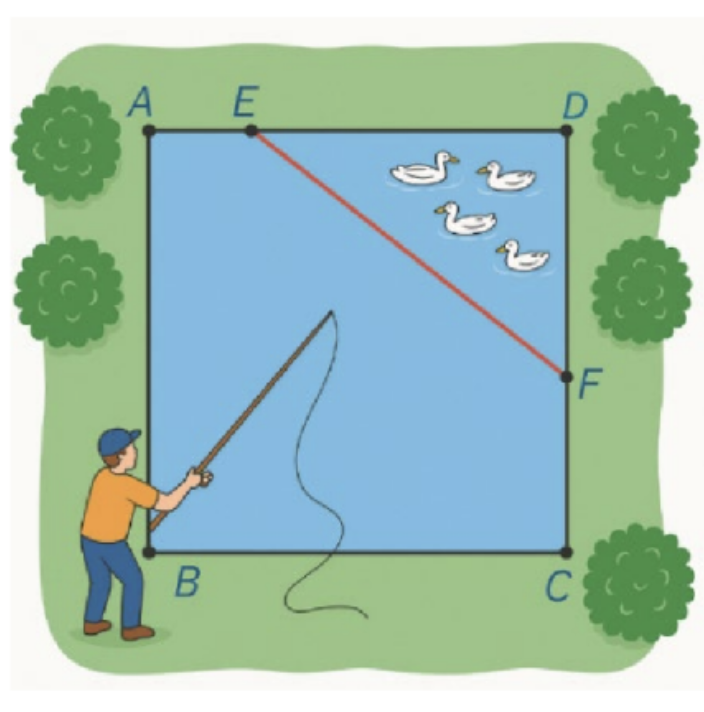
\includegraphics[width=0.3\textwidth]{5.10.png}
\end{center}
\textbf{Câu 2.} Một gương hypebol (được sử dụng trong một số kính thiên văn) có tính chất là một tia sáng hướng vào tiêu điểm sẽ bị phản xạ sang tiêu điểm khác. Gương trong hình vẽ có phương trình $\dfrac{x^2}{36} - \dfrac{y^2}{64} = 1$. Điểm $M(a; b)$ trên gương sẽ nhận được tia sáng đi qua điểm $(0; 10)$ và bị phản xạ sang tiêu điểm còn lại? (tham khảo hình vẽ).\\
a) Độ dài trục thực của gương là $12$.\\
b) Tiêu cự của gương là $10$.\\
c) Phương trình đường thẳng tia sáng $y = -x + 10$.\\
d) Giá trị $T = a + b$ lớn hơn $10$.\\
\vspace{0.5cm}
\begin{center}
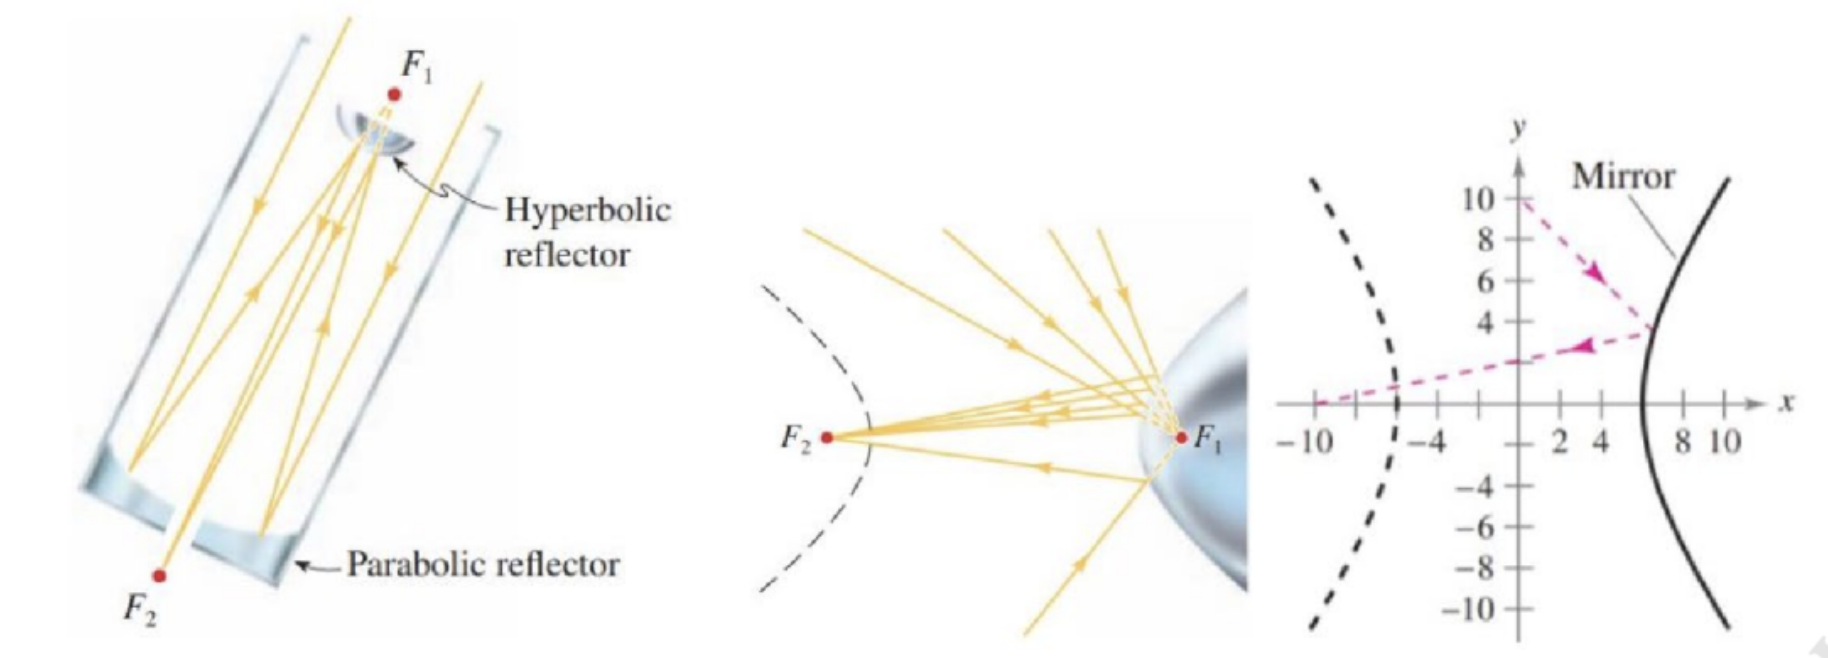
\includegraphics[width=0.5\textwidth]{6.2.png}
\end{center}
\textbf{Câu 4.} Một cây cầu vòm chịu lực hình nửa Elip dựng trên con sông nhỏ có chiều rộng $20$ m. Điểm giữa của vòm cách mặt nước $6m$. Phương trình chính tắc của elip với trục hoành ở vị trí mặt nước và trục tung đi qua điểm chính giữa của vòm có dạng $\dfrac{x^2}{a^2} + \dfrac{y^2}{b^2} = 1(0 < b < a)$.
Tính $a^2 + b^2$.
\begin{center}

\includegraphics[width=0.5\textwidth]{6.4.png}
\end{center}
$\Rightarrow$ Đáp số: ..........
\end{document}